The Core Logic Layer subsystems are centered around planning and executing the main actions needed by the machine. 

\subsection{Command Pipeline}
The Command Pipeline is a ordered que of actions which are known to need execution. Each action is read off the top of the list and executed at an indicated time. The command pipeline must also assign an action to the appropriate system for execution.

\begin{figure}[h!]
	\centering
 	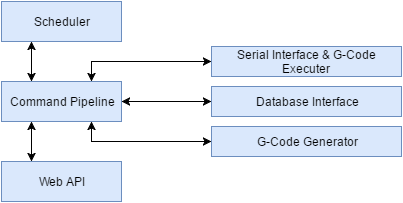
\includegraphics[width=0.60\textwidth]{images/core_logic_layer}
 \caption{Example subsystem description diagram}
\end{figure}

\subsubsection{Assumptions}
The command pipeline assumes that the other system components are always available to execute commands. 

\subsubsection{Responsibilities}
The command pipeline must accurately maintain the order of execution for its tasks.

\subsubsection{Subsystem Interfaces}
The command pipeline must be able to interface with all the other systems it executes commands for. The primary interface for these transactions is through a html web API. 

\begin {table}[H]
\caption {Subsystem interfaces} 
\begin{center}
    \begin{tabular}{ | p{1cm} | p{6cm} | p{3cm} | p{3cm} |}
    \hline
    ID & Description & Inputs & Outputs \\ \hline
    \#01 & Scheduler bus & \pbox{3cm}{Upcomming task events} & \pbox{3cm}{Future Actions needed}  \\ \hline
    \#02 & Serial Pipeline & \pbox{3cm}{Serial Data} & \pbox{3cm}{Serial Commands}  \\ \hline
    \#03 & G-Code interface & \pbox{3cm}{Serial Data} & \pbox{3cm}{Serial Commands}  \\ \hline
    \end{tabular}
\end{center}
\end{table}

\subsection{Scheduler}
The Scheduler subsystem is built to store requested command events as well as request their timely execution by the command pipeline

\subsubsection{Assumptions}
The scheduler is assumed to be constantly running. 

\subsubsection{Responsibilities}
The primary purpose of the scheduler was to ensure commands have been executed in a timely manner. This necessitates an internal time tracking system to ensure commands are being executed when they are scheduled to.

\subsubsection{Subsystem Interfaces}
The scheduler subsystem only needs to interface directly with the command pipeline. It must be able to send and recieve full command instructions as used by the command pipeline.

\begin {table}[H]
\caption {Subsystem interfaces} 
\begin{center}
    \begin{tabular}{ | p{1cm} | p{6cm} | p{3cm} | p{3cm} |}
    \hline
    ID & Description & Inputs & Outputs \\ \hline
    \#01 & Scheduler bus & \pbox{3cm}{Upcoming  task events} & \pbox{3cm}{Future Actions needed}  \\ \hline
    \end{tabular}
\end{center}
\end{table}

\subsection{Web API}
The Web API subsystem is to allow interfacing to the rest of the FarmBot systems.

\subsubsection{Assumptions}
The Web API subsystem is assumed to not need user authentication for security. 

\subsubsection{Responsibilities}
The Web API subsystem must listen for input from other layers within the FarmBot architecture. If the input is not provided in a sensible manner, it must be transformed in the subsystem. 

\subsubsection{Subsystem Interfaces}
The Web API subsystem provides an unsecured html interface. 

\begin {table}[H]
\caption {Subsystem interfaces} 
\begin{center}
    \begin{tabular}{ | p{1cm} | p{6cm} | p{3cm} | p{3cm} |}
    \hline
    ID & Description & Inputs & Outputs \\ \hline
    \#01 & HTML & \pbox{3cm}{html requests} & \pbox{3cm}{html responses}  \\ \hline
    \end{tabular}
\end{center}
\end{table}

\subsection{Database Interface}
The Database Interface subsystem allows data transactions to the central database. 

\subsubsection{Assumptions}
The data passing though the database interface is assumed to be in the final form required before storing. The Database Layer may not always be available.

\subsubsection{Responsibilities}
The database interface must attempt to send data to the Database Layer of the FarmBot. Data which cannot immediately be pushed to the data layer will be buffered within the subsystem until a timeout or the Database Layer accepts the data.

\subsubsection{Subsystem Interfaces}
The Database interface only communicates to the command pipeline subsystem and the database layer API. 

\begin {table}[H]
\caption {Subsystem interfaces} 
\begin{center}
    \begin{tabular}{ | p{1cm} | p{6cm} | p{3cm} | p{3cm} |}
    \hline
    ID & Description & Inputs & Outputs \\ \hline
    \#01 & Command Pipeline & \pbox{3cm}{Data store requests} & \pbox{3cm}{responses}  \\ \hline
    \end{tabular}
\end{center}
\end{table}

\subsection{G-Code Generator}
The G-Code generator subsystem is the software element which converts command actions in the pipeline into executable machine movement code.  

\subsubsection{Assumptions}
The development of this subsystem assumes that complex actions can be consistently digested into a series of motor control actions. 

\subsubsection{Responsibilities}
The G-Code generator will be responsible for creating all motor control actions. 

\subsubsection{Subsystem Interfaces}
The G-Code Generator only communicates to the command pipeline subsystem.

\begin {table}[H]
\caption {Subsystem interfaces} 
\begin{center}
    \begin{tabular}{ | p{1cm} | p{6cm} | p{3cm} | p{3cm} |}
    \hline
    ID & Description & Inputs & Outputs \\ \hline
    \#01 & Command Pipeline & \pbox{3cm}{Actions} & \pbox{3cm}{G-Code Commands}  \\ \hline
    \end{tabular}
\end{center}
\end{table}

\subsection{Serial Interface}
The serial interface connects the core logic layer to the motor control layer.

\subsubsection{Assumptions}
We are assuming the motor control layer requires no input from the rest of the systems beyond coordinate actions. We are also assuming the motor control layer acknowledges receiving all instructions and if no response is received by the motor control layer the instruction was unable to be executed.

\subsubsection{Responsibilities}
The Serial Interface is responsible for parsing action in the command pipeline sending them to the motor control layer. 

\subsubsection{Subsystem Interfaces}
The Serial Interface only communicates to the command pipeline subsystem and the motor control layer.

\begin {table}[H]
\caption {Subsystem interfaces} 
\begin{center}
    \begin{tabular}{ | p{1cm} | p{6cm} | p{3cm} | p{3cm} |}
    \hline
    ID & Description & Inputs & Outputs \\ \hline
    \#01 & Command Pipeline & \pbox{3cm}{G-Code Commands} & \pbox{3cm}{Serial Strings}  \\ \hline
    \end{tabular}
\end{center}
\end{table}